\section{Image cleaning: Tailcuts vs. FACT}

\begin{frame}
    \centering
    {\Huge \textbf{Image cleaning in FACT}}
\end{frame}

\begin{frame}{Cleaning Methods}
    \begin{columns}[T] % align columns
        \begin{column}{.48\textwidth}
            \textbf{Tailcuts cleaning}
            \vspace{8pt}
            \begin{itemize}
                \item "Two treshold procedure"
                \item Pixels above upper threshold survive
                \item Signal pixels need at least N neighbors
                \item Add neighboring pixels above the lower threshold
            \end{itemize}
        \end{column}
        \begin{column}{.48\textwidth}
            \textbf{"FACT image cleaning"}
            \vspace{8pt}
            \begin{itemize}
                \item Similar behaviour, but also uses information about the arrival times
                \item Pixels nedd to have a similar arrival time as their neighbors
                \item More steps removing "lonely" pixels
                \item[\rightarrow] Probably removes more pixels with the same intensity thresholds
            \end{itemize}
        \end{column}
    \end{columns}
\end{frame}

\begin{frame}{Sample MC Event}
    \begin{figure}
        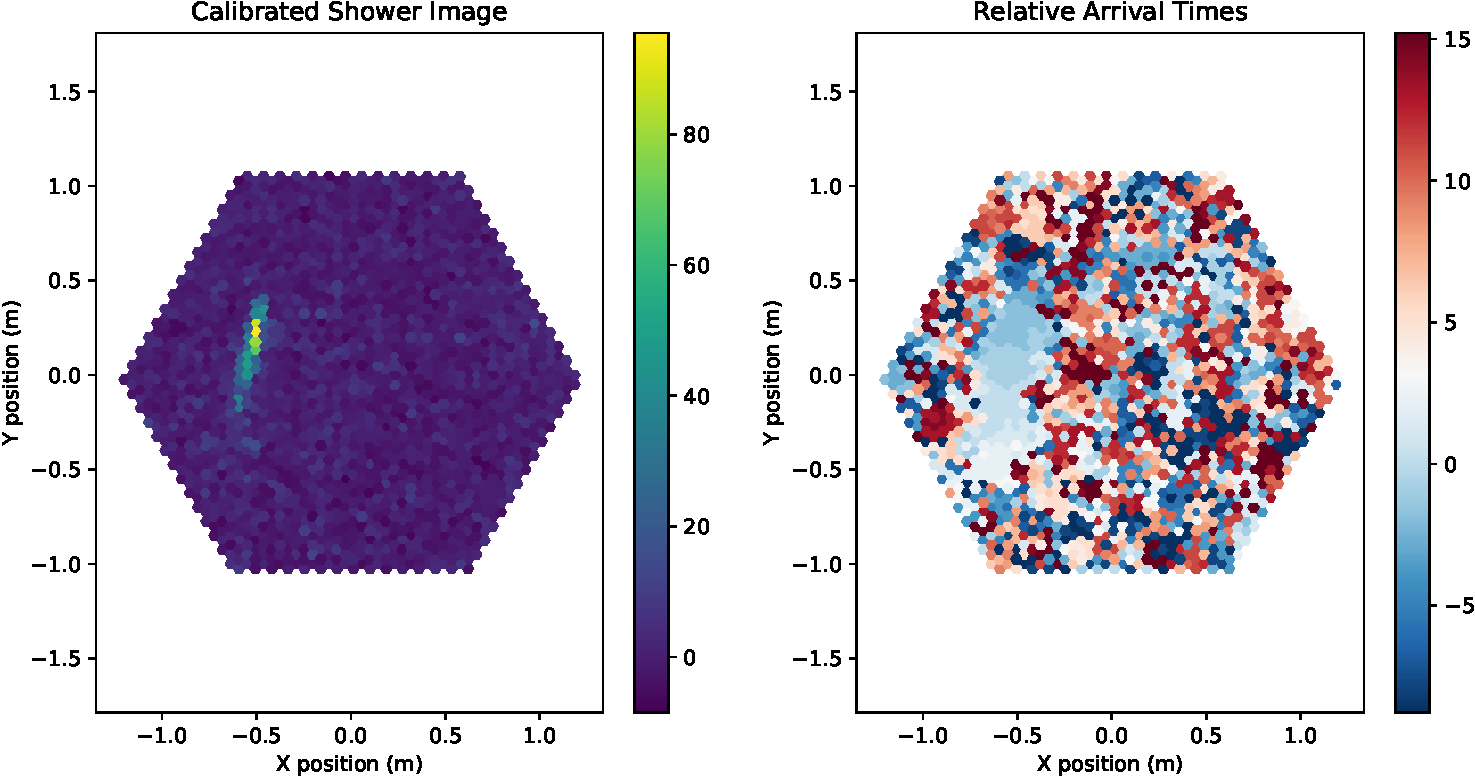
\includegraphics[width=0.85\linewidth]{images/cleaning_plots/raw-crop.pdf}
    \end{figure}
\end{frame}



% \begin{frame}{Sample MC event on a Flash Cam}
%     \begin{itemize}
%         \item cleaning levels from LST Cam
%         \item unoptimized for the Flash Cam
%         \item intensity thresholds far too low
%         \item bad cleaning performance expected
%     \end{itemize}
% \end{frame}


% \begin{frame}{Cleaning: Tailcuts approach}
%     \begin{figure}
%         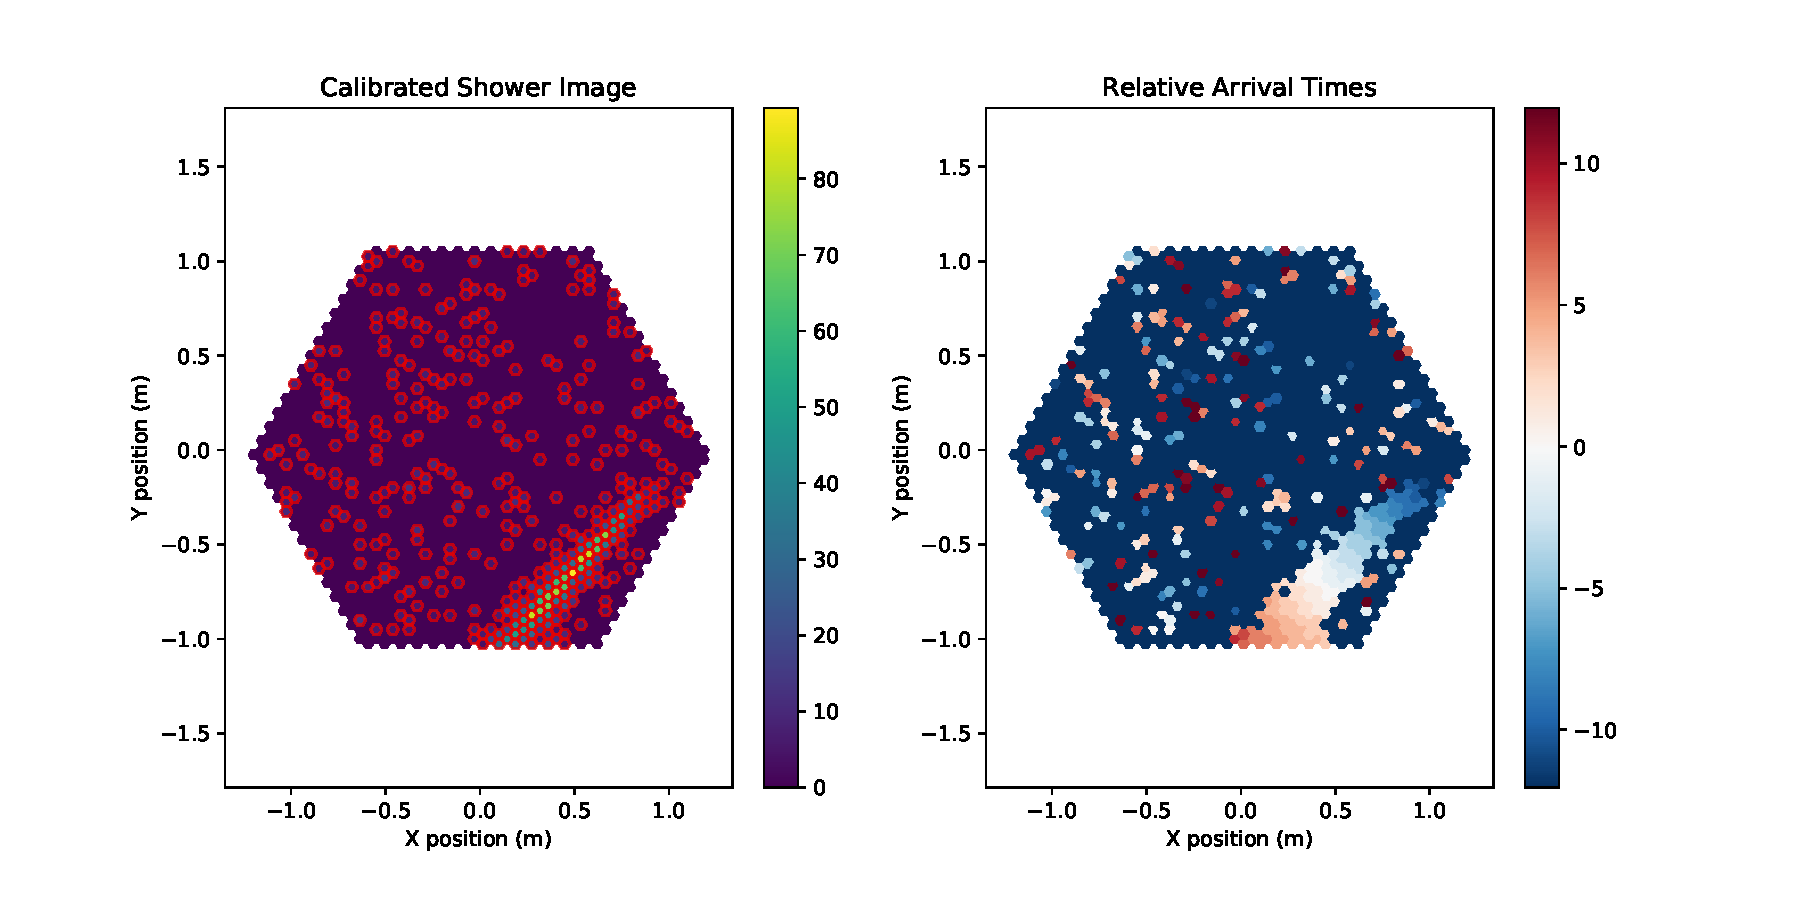
\includegraphics[width=\linewidth]{images/cleaning_plots/tail_1.pdf}
%     \end{figure}
% \end{frame}

% \begin{frame}{Cleaning: Tailcuts approach}
%     \begin{figure}
%         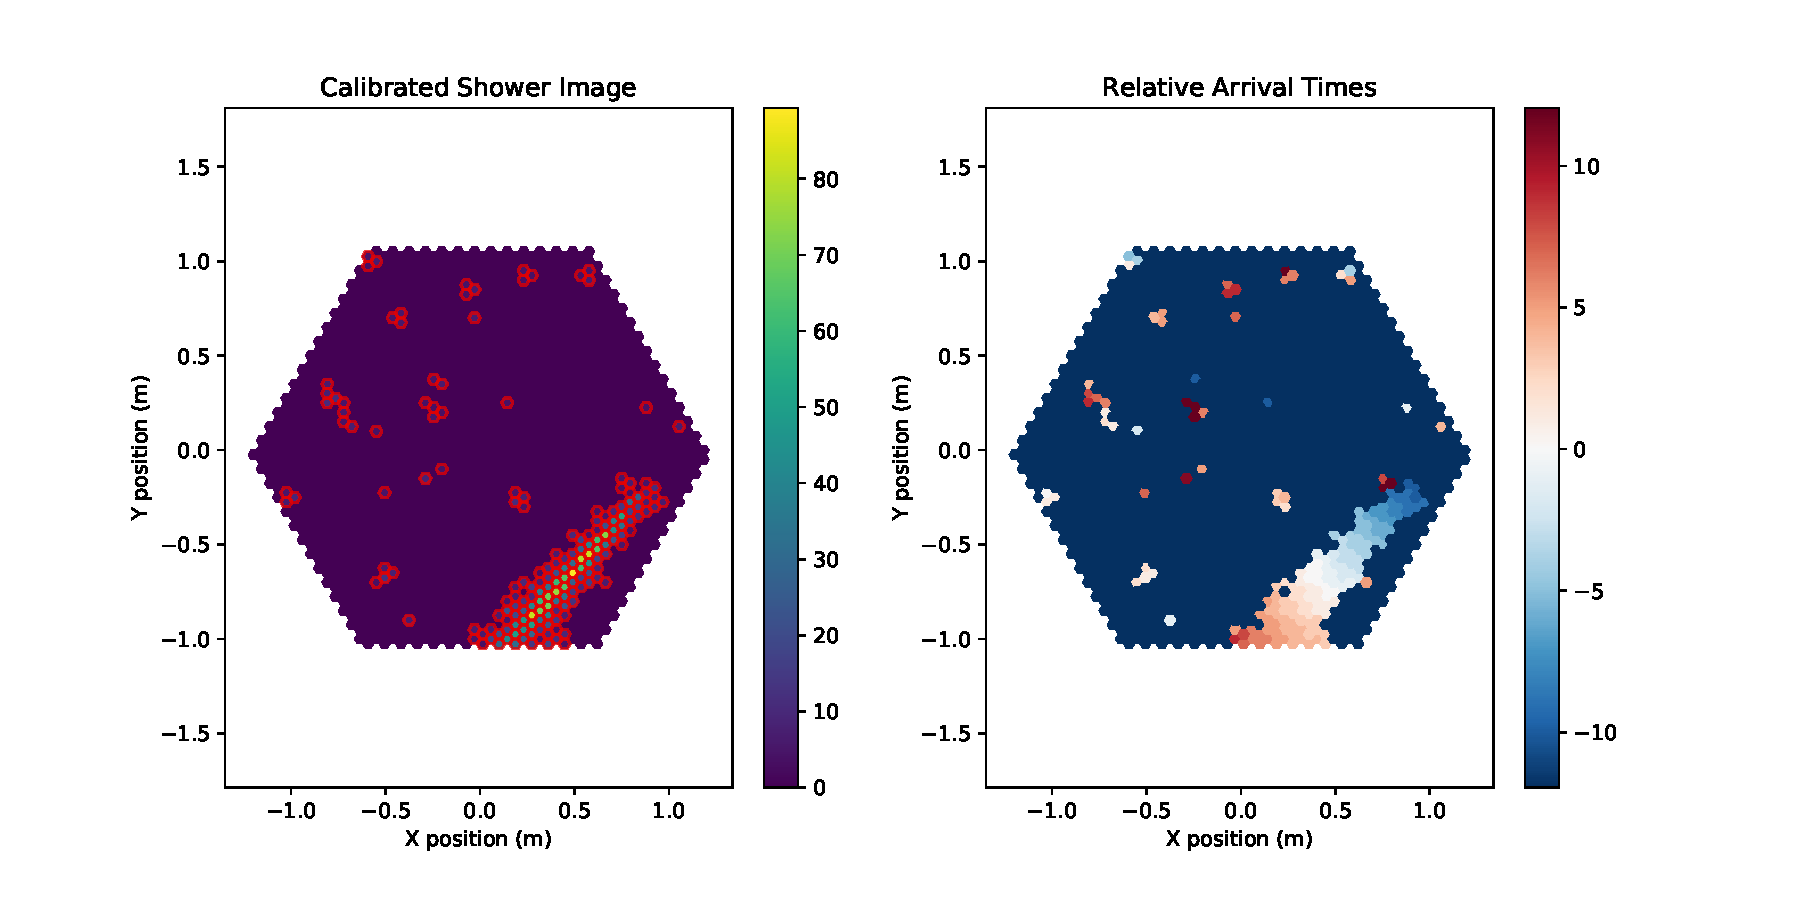
\includegraphics[width=\linewidth]{images/cleaning_plots/tail_2.pdf}
%     \end{figure}
% \end{frame}

% \begin{frame}{Cleaning: Tailcuts approach}
%     \begin{figure}
%         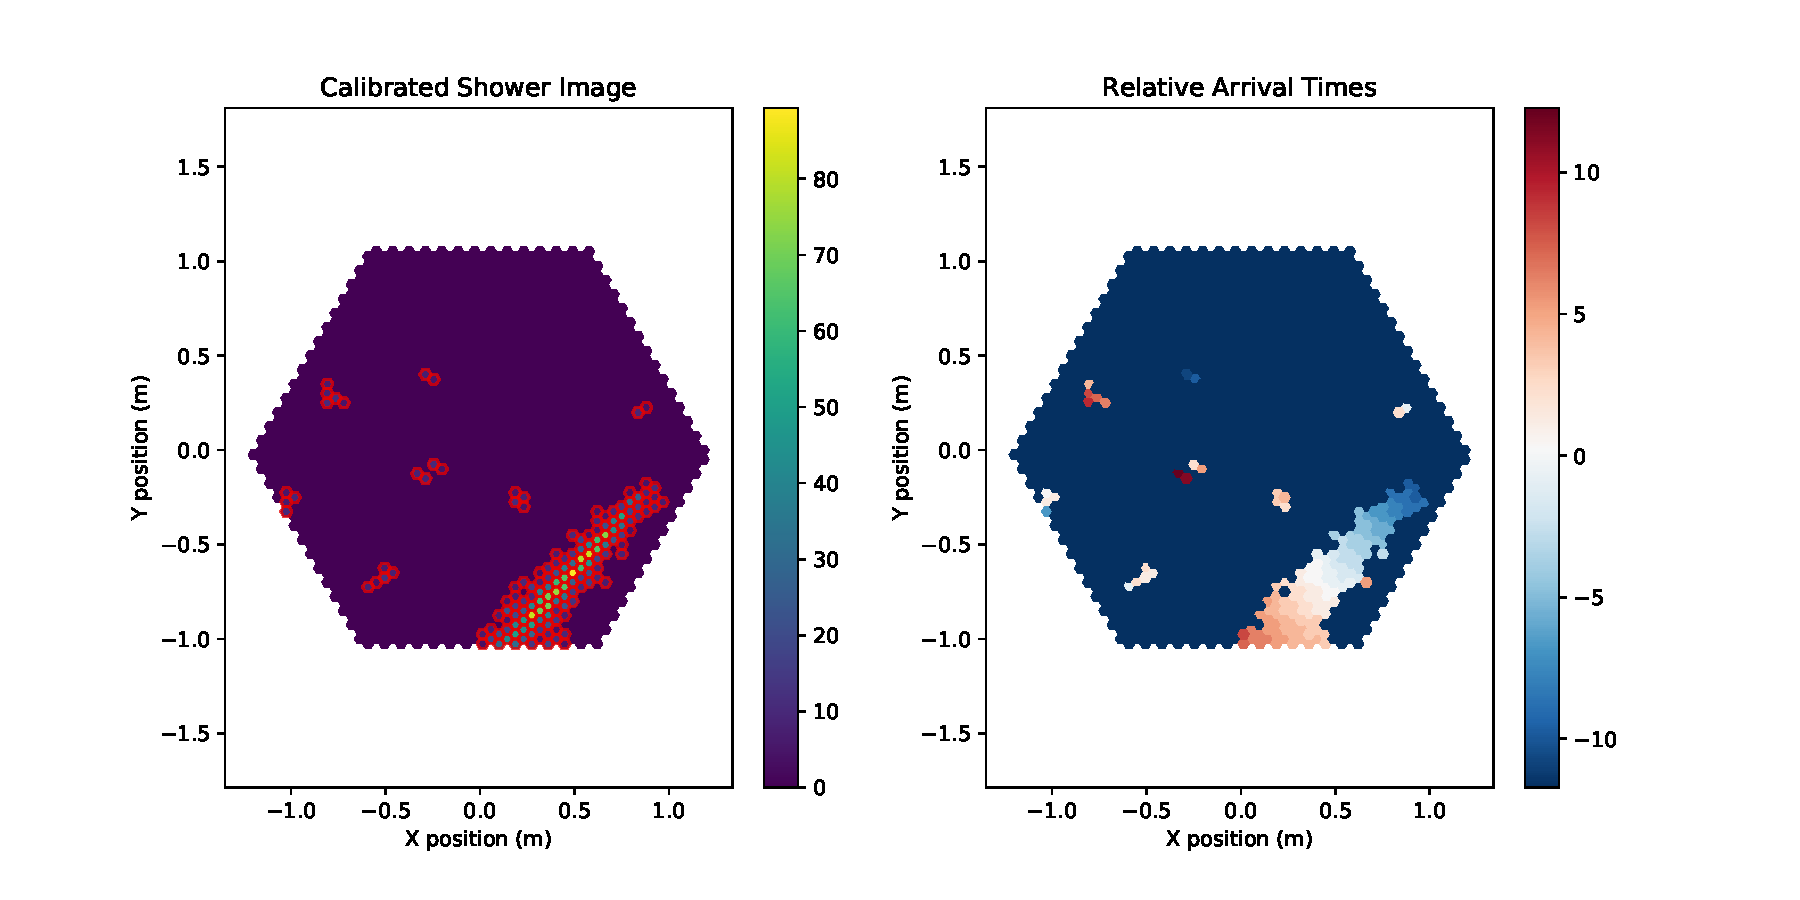
\includegraphics[width=\linewidth]{images/cleaning_plots/tail_3.pdf}
%     \end{figure}
% \end{frame}

% \begin{frame}{Cleaning: FACT approach}
%     \begin{figure}
%         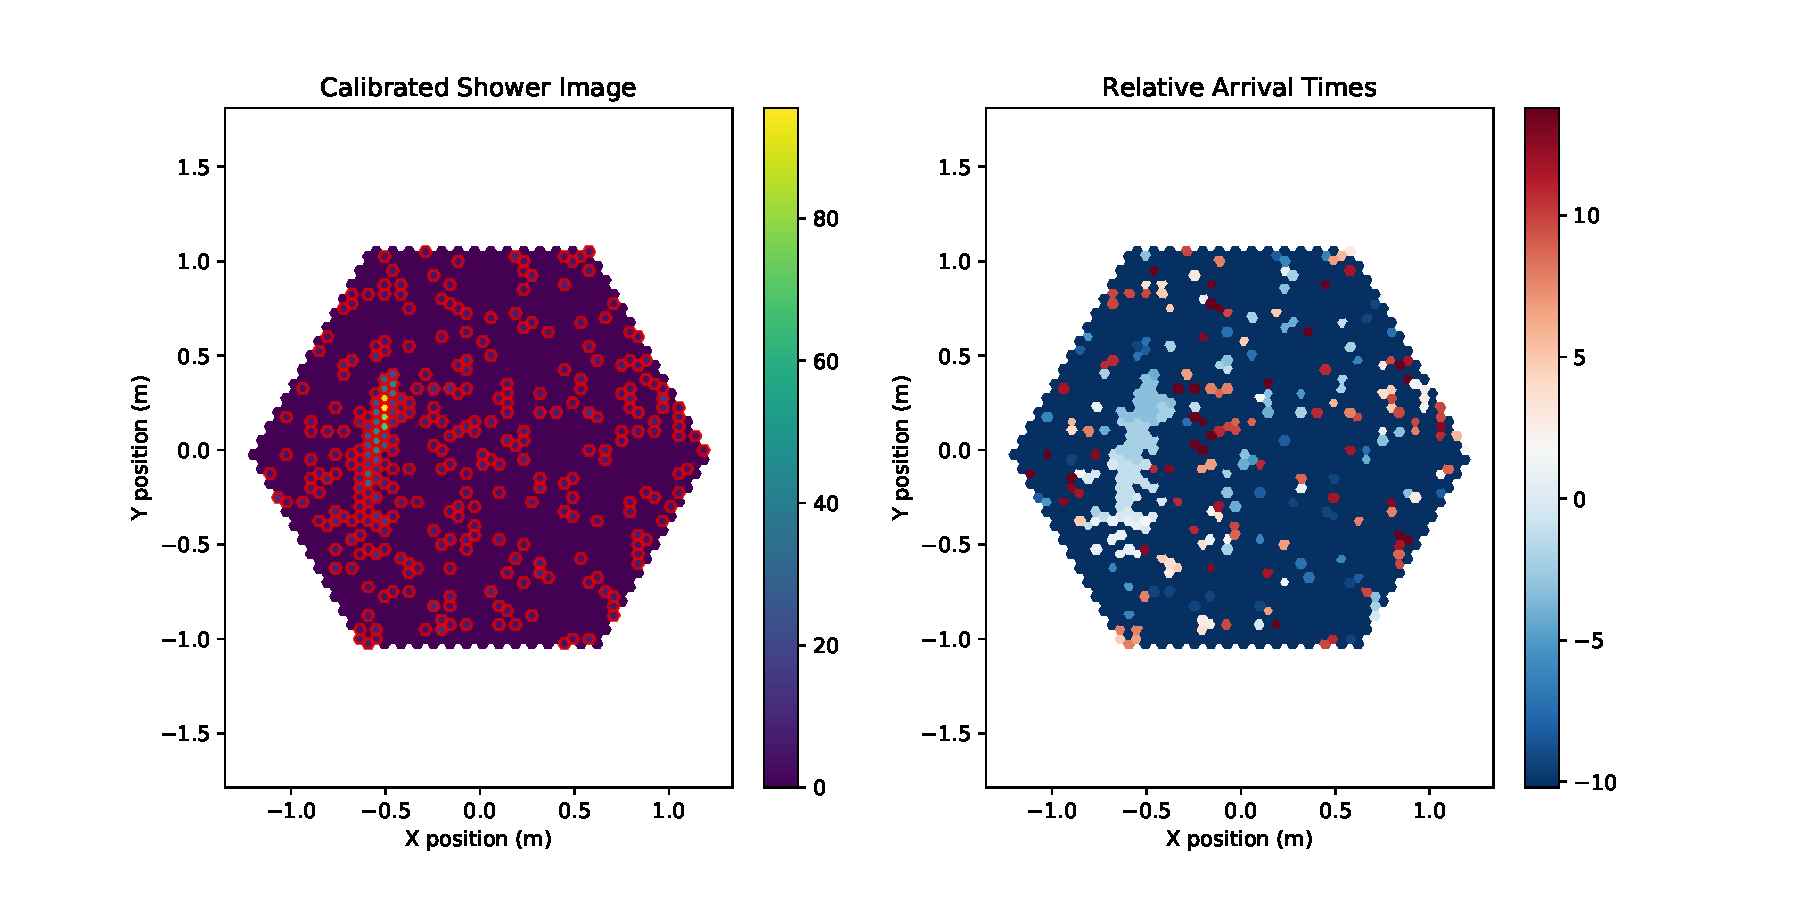
\includegraphics[width=\linewidth]{images/cleaning_plots/fact_1.pdf}
%     \end{figure}
% \end{frame}

% \begin{frame}{Cleaning: FACT approach}
%     \begin{figure}
%         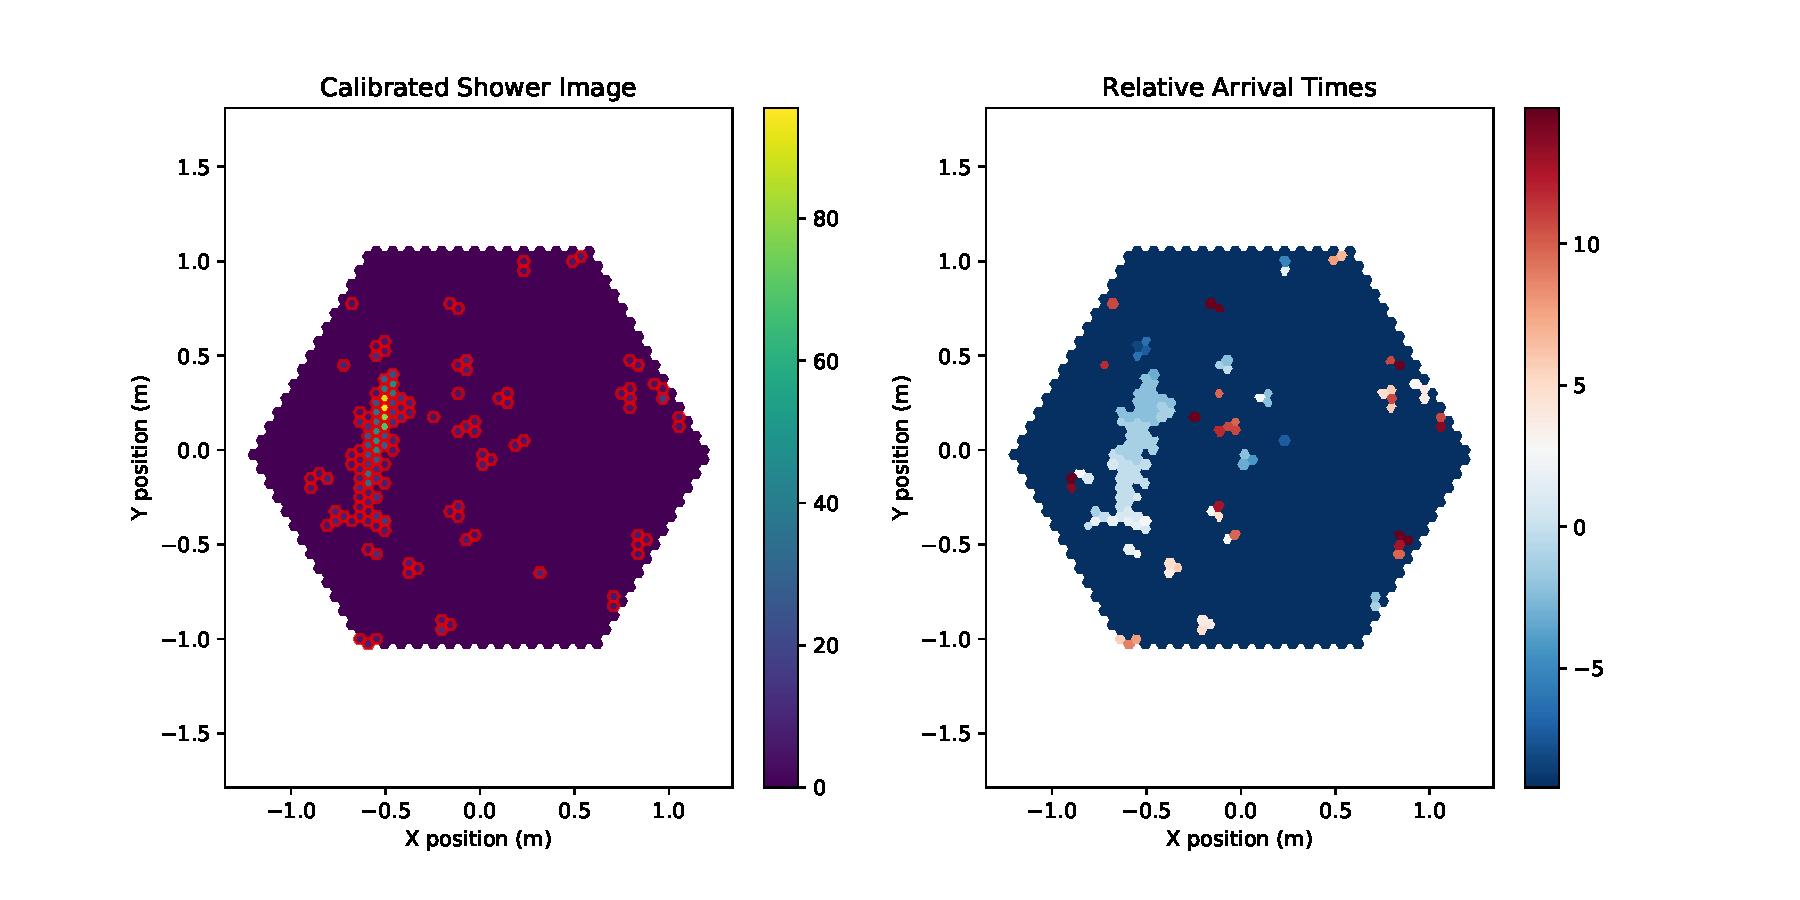
\includegraphics[width=\linewidth]{images/cleaning_plots/fact_2.pdf}
%     \end{figure}
% \end{frame}

% \begin{frame}{Cleaning: FACT approach}
%     \begin{figure}
%         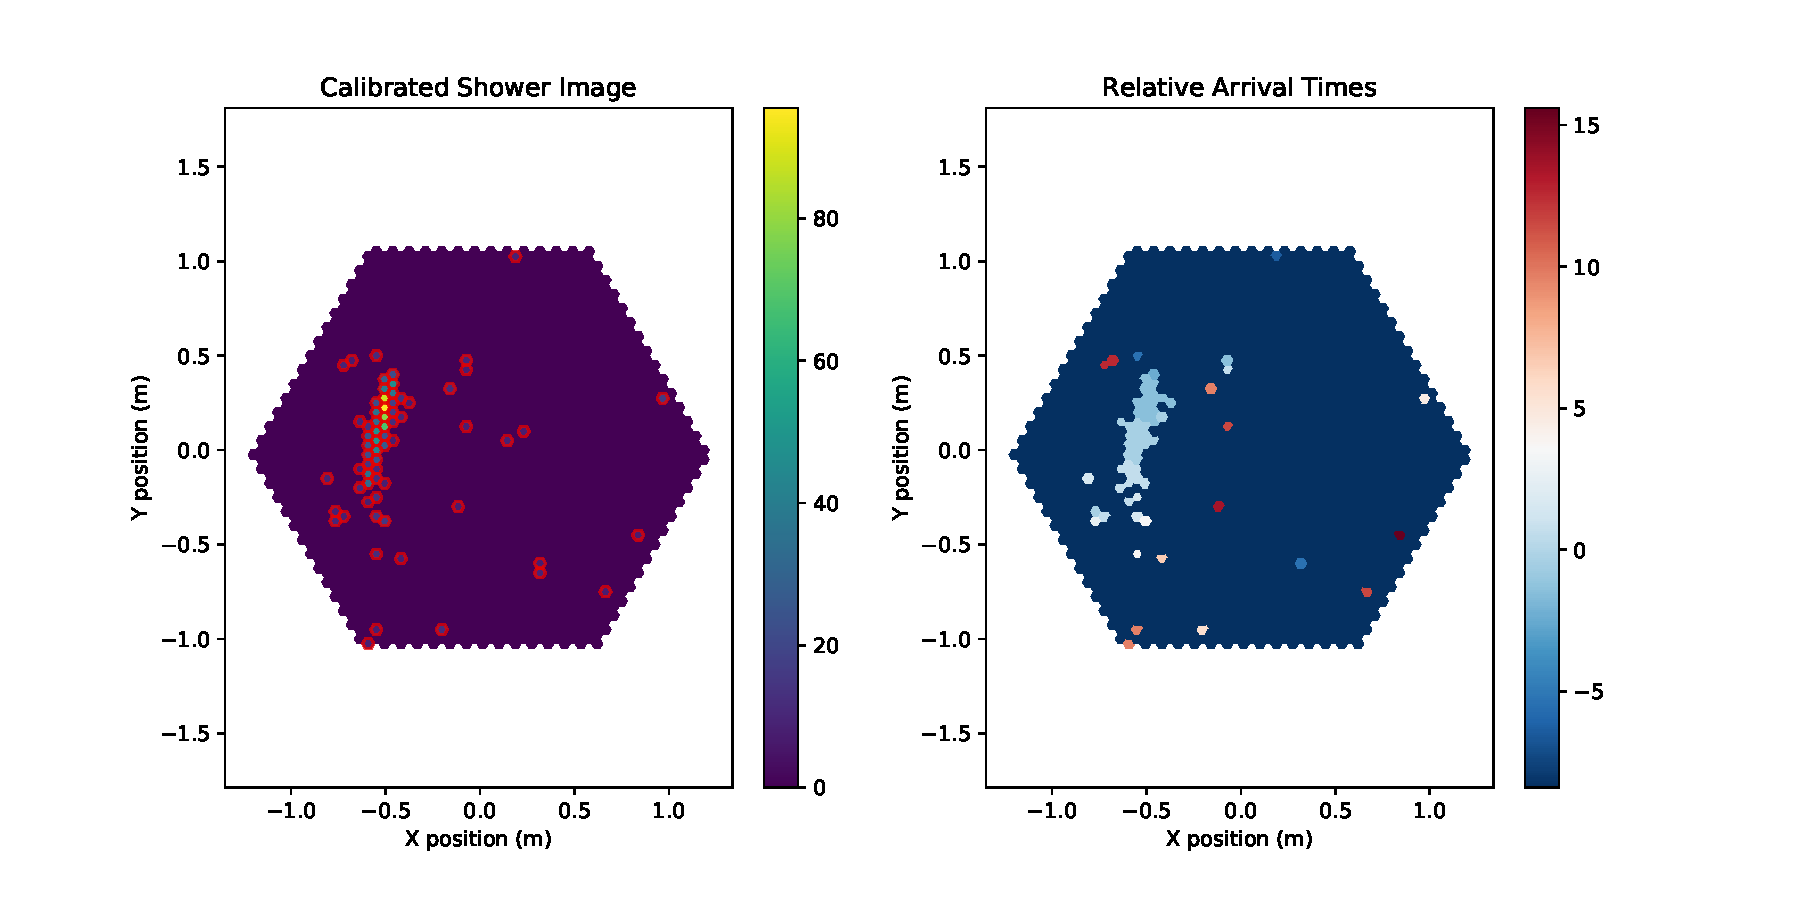
\includegraphics[width=\linewidth]{images/cleaning_plots/fact_3.pdf}
%     \end{figure}
% \end{frame}

% \begin{frame}{Cleaning: FACT approach}
%     \begin{figure}
%         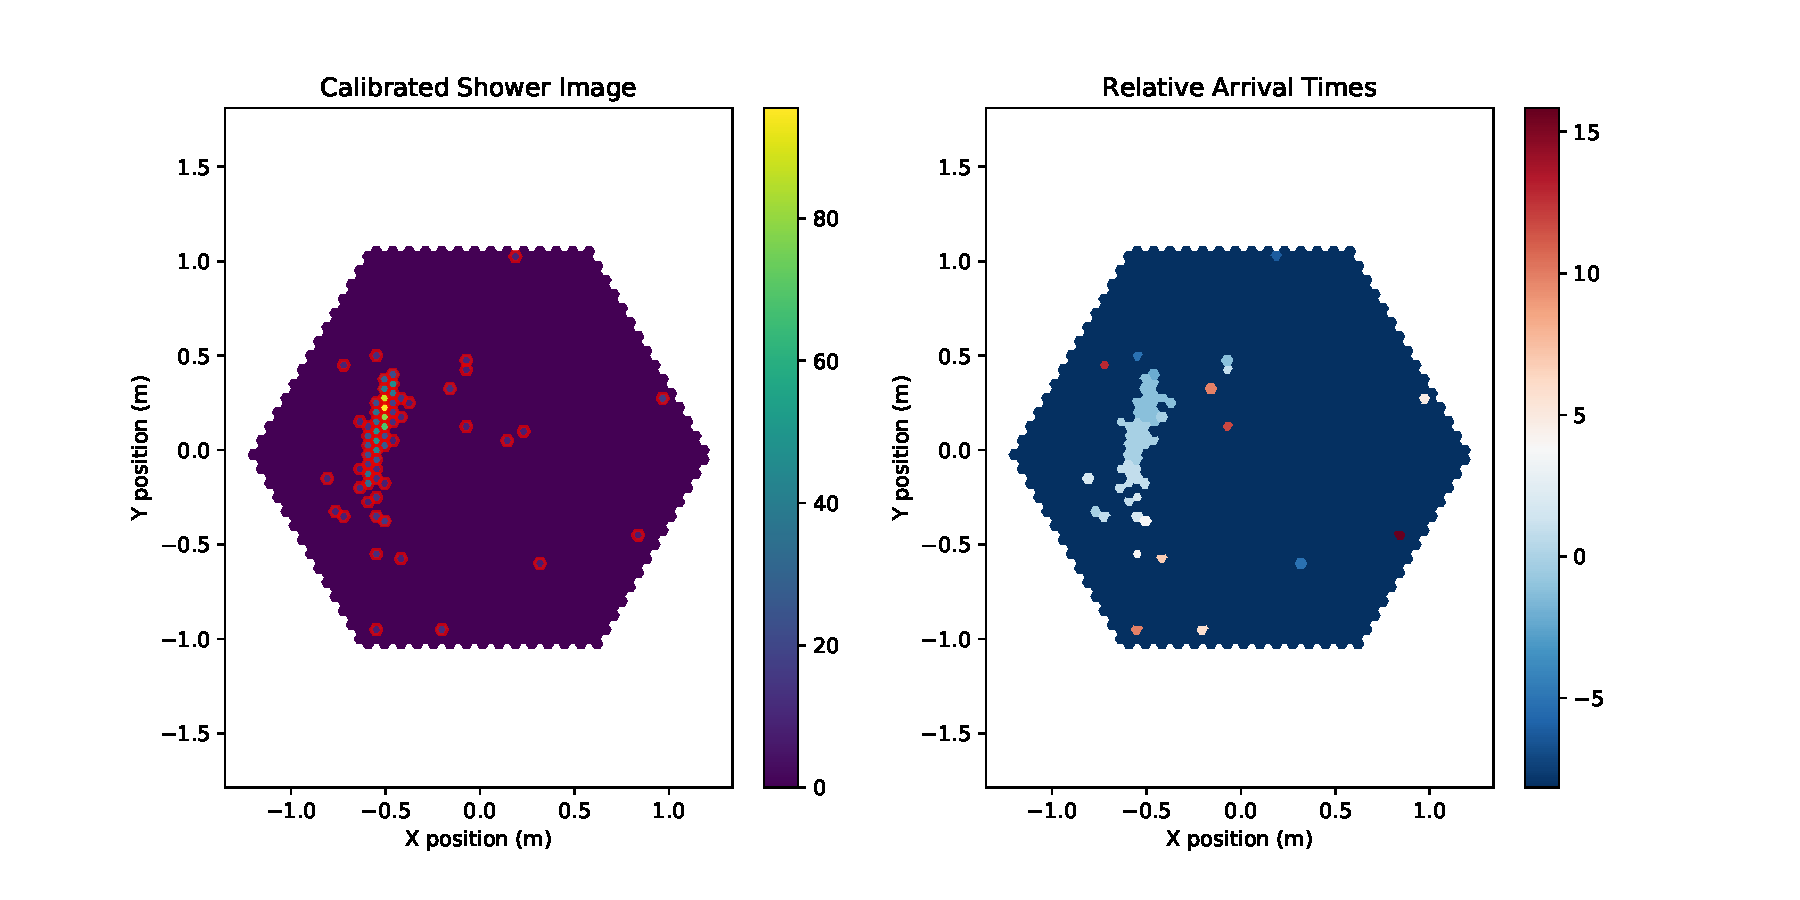
\includegraphics[width=\linewidth]{images/cleaning_plots/fact_4.pdf}
%     \end{figure}
% \end{frame}

% \begin{frame}{Cleaning: FACT approach}
%     \begin{figure}
%         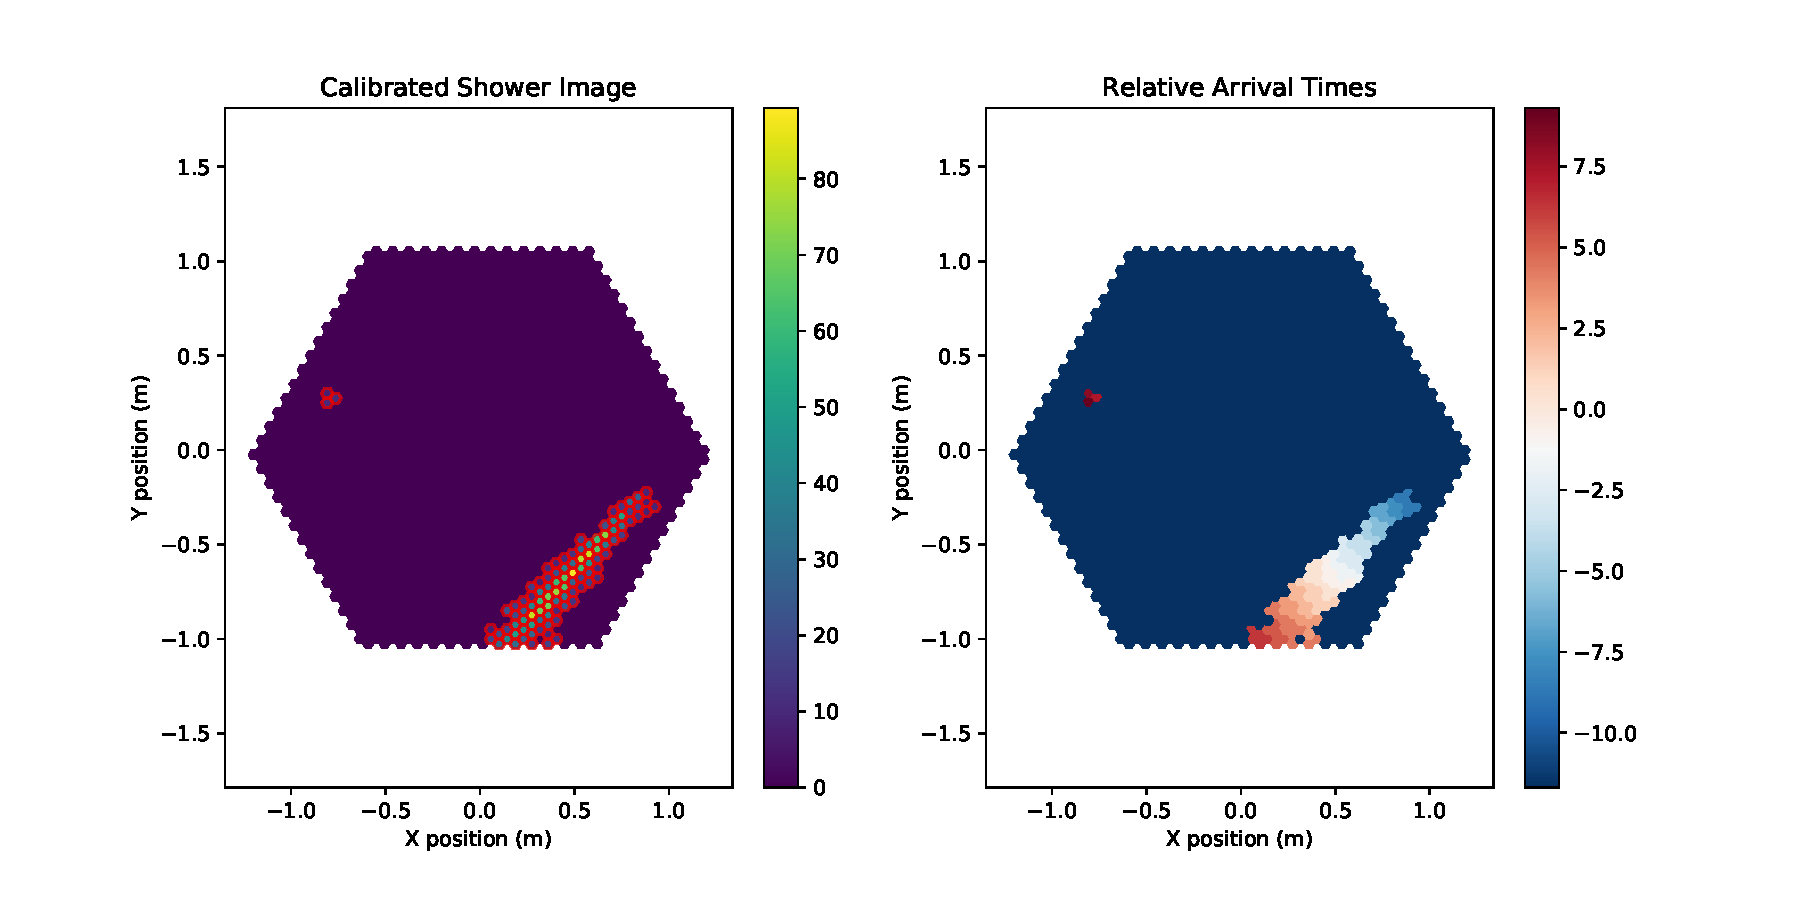
\includegraphics[width=\linewidth]{images/cleaning_plots/fact_5.pdf}
%     \end{figure}
% \end{frame}

% \begin{frame}{Cleaning: FACT approach}
%     \begin{figure}
%         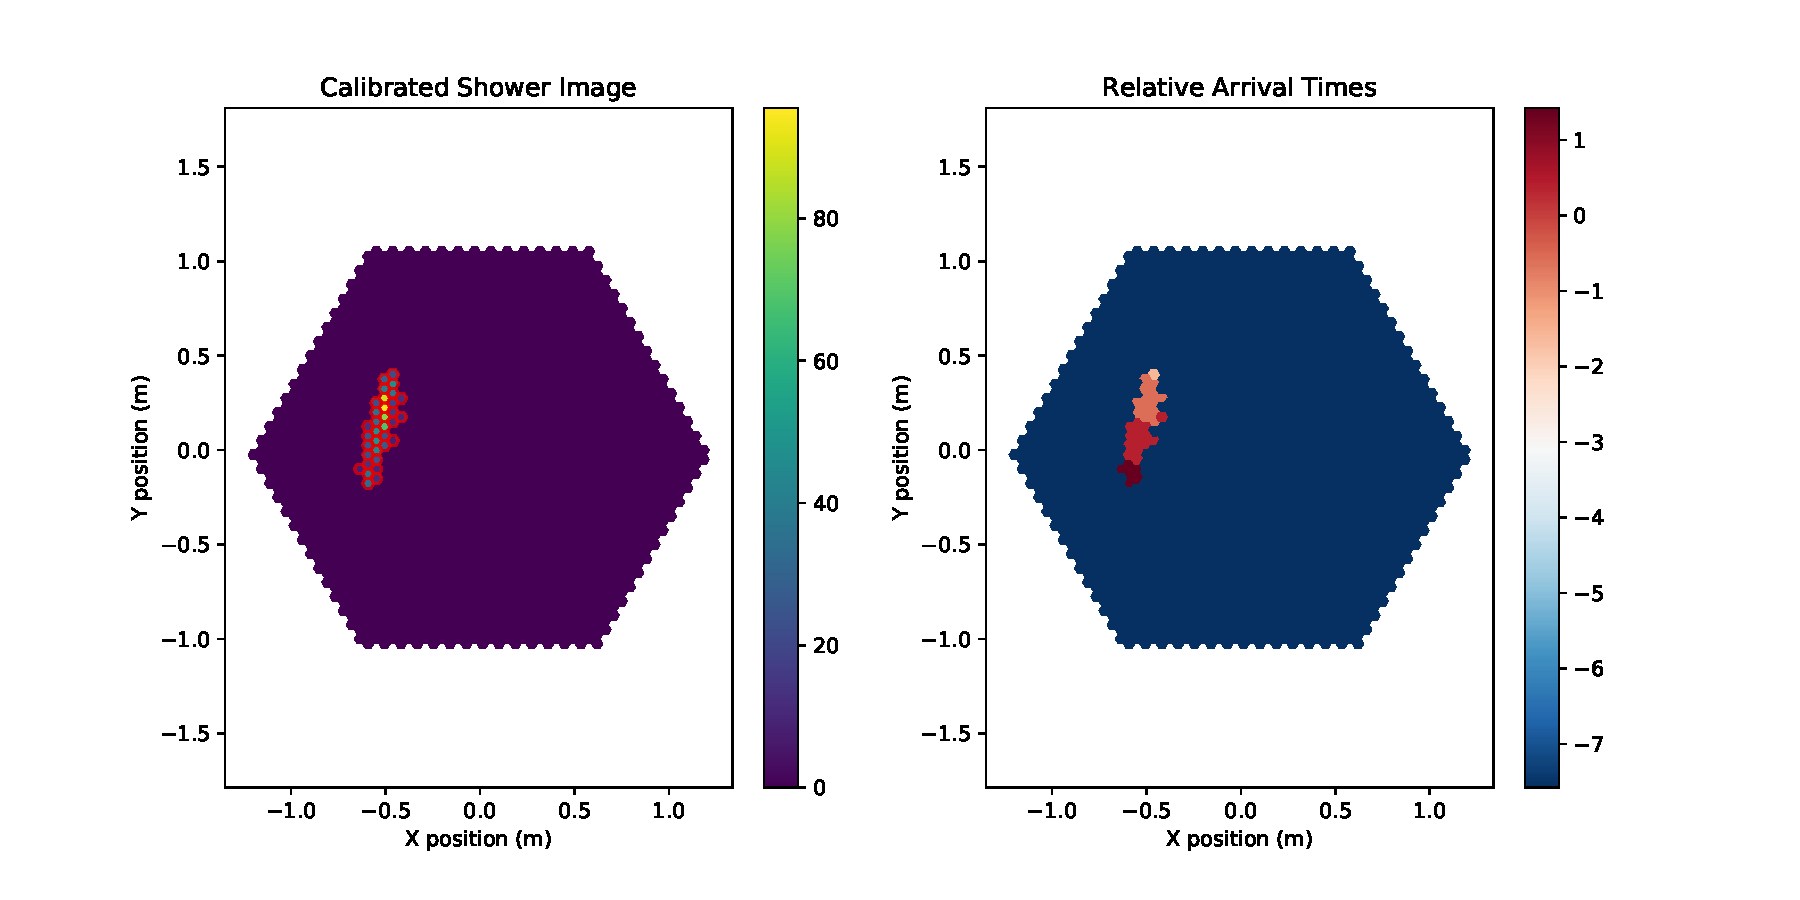
\includegraphics[width=\linewidth]{images/cleaning_plots/fact_6.pdf}
%     \end{figure}
% \end{frame}

\begin{frame}{Cleaning Results}
    \begin{figure}
        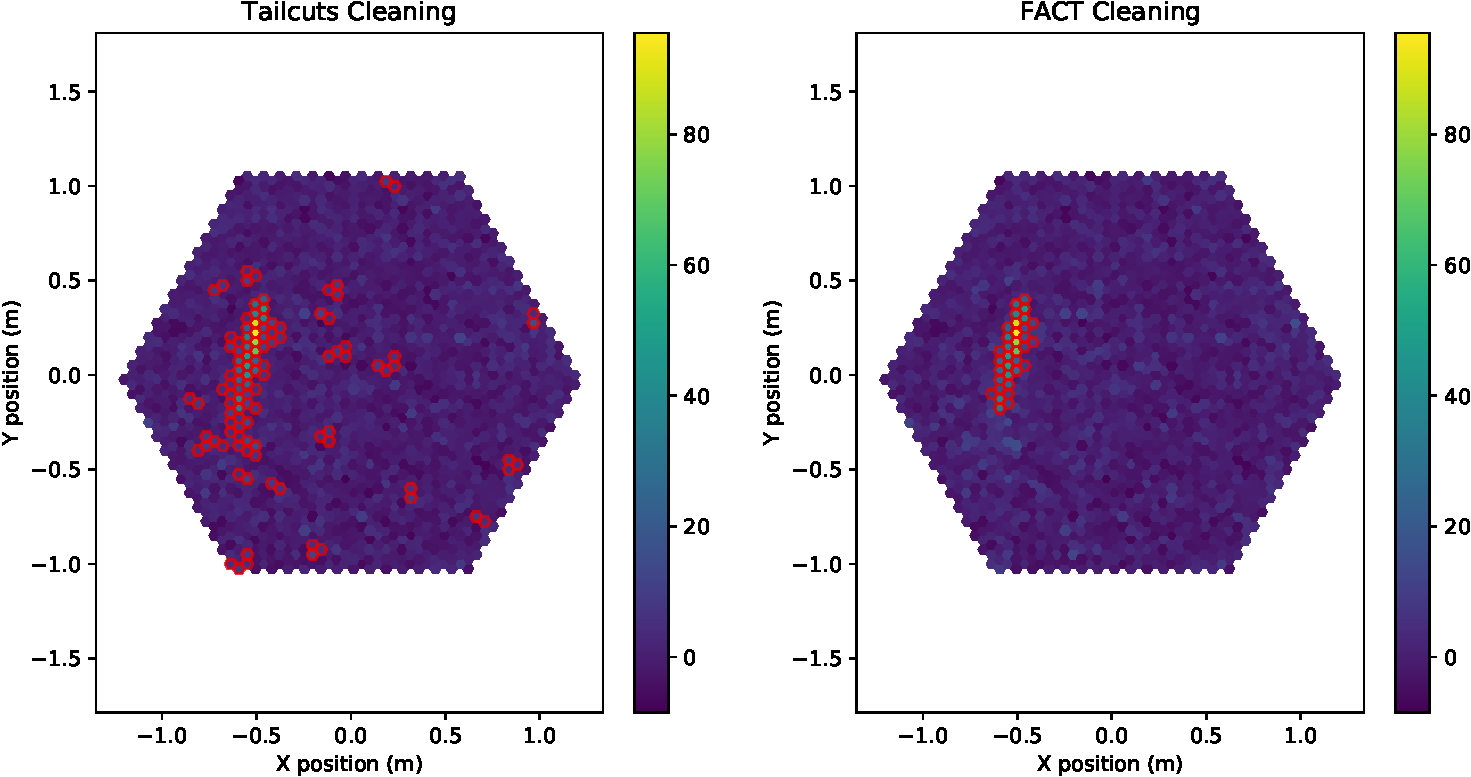
\includegraphics[width=0.85\linewidth]{images/cleaning_plots/comparison-crop.pdf}
    \end{figure}
\end{frame}